\documentclass[tikz]{standalone}
\usetikzlibrary{arrows.meta,math}
\usepackage{xcolor}
\begin{document}
	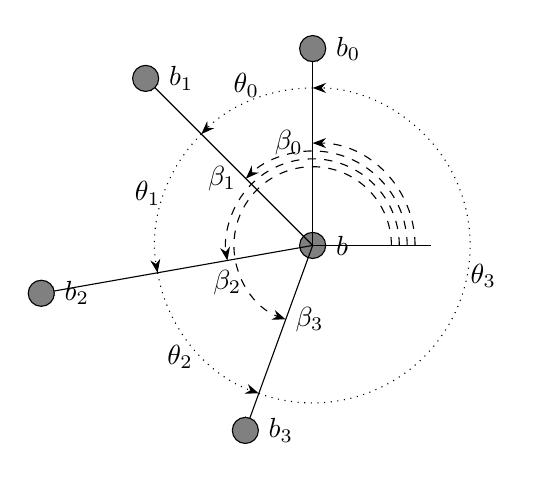
\begin{tikzpicture}[>=Stealth]
	\node[circle,fill=black!50,draw,label=right:$b$]{};
	\draw (0,0)--(right:1.5cm);
	\foreach \n/\d/\l/\a/\r/\p in { 
			0/1.3cm/b_0/90/2.5cm/left, 
			1/1.2cm/b_1/135/3cm/left,
			2/1.1cm/b_2/190/3.5cm/below,
			3/1.0cm/b_3/250/2.5cm/right}
		{
		\draw[->] (0,0)--node[above,sloped, very near end]{} (\a:\r) 
					node[circle,fill=black!50,draw,label=right:$\l$]{};
		\draw[->,dashed] (\d, 0) arc[start angle=0, delta angle=\a,
		radius=\d] node[\p]{$\beta_\n$};
	};

	\foreach \n/\b/\t in { 0/90/135 , 1/135/190 , 2/190/250 , 3/250/450 } {
		\draw[dotted,->] (\b:2cm) arc[start angle=\b, delta angle=\t-\b,radius=2cm];
		\draw (\b/2+\t/2:2.2cm) node {$\theta_\n$};
	};
	\end{tikzpicture}
\end{document}

